% Options for packages loaded elsewhere
\PassOptionsToPackage{unicode}{hyperref}
\PassOptionsToPackage{hyphens}{url}
%
\documentclass[
]{article}
\usepackage{lmodern}
\usepackage{amssymb,amsmath}
\usepackage{ifxetex,ifluatex}
\ifnum 0\ifxetex 1\fi\ifluatex 1\fi=0 % if pdftex
  \usepackage[T1]{fontenc}
  \usepackage[utf8]{inputenc}
  \usepackage{textcomp} % provide euro and other symbols
\else % if luatex or xetex
  \usepackage{unicode-math}
  \defaultfontfeatures{Scale=MatchLowercase}
  \defaultfontfeatures[\rmfamily]{Ligatures=TeX,Scale=1}
\fi
% Use upquote if available, for straight quotes in verbatim environments
\IfFileExists{upquote.sty}{\usepackage{upquote}}{}
\IfFileExists{microtype.sty}{% use microtype if available
  \usepackage[]{microtype}
  \UseMicrotypeSet[protrusion]{basicmath} % disable protrusion for tt fonts
}{}
\makeatletter
\@ifundefined{KOMAClassName}{% if non-KOMA class
  \IfFileExists{parskip.sty}{%
    \usepackage{parskip}
  }{% else
    \setlength{\parindent}{0pt}
    \setlength{\parskip}{6pt plus 2pt minus 1pt}}
}{% if KOMA class
  \KOMAoptions{parskip=half}}
\makeatother
\usepackage{xcolor}
\IfFileExists{xurl.sty}{\usepackage{xurl}}{} % add URL line breaks if available
\IfFileExists{bookmark.sty}{\usepackage{bookmark}}{\usepackage{hyperref}}
\hypersetup{
  pdftitle={Final Project},
  hidelinks,
  pdfcreator={LaTeX via pandoc}}
\urlstyle{same} % disable monospaced font for URLs
\usepackage[margin=1in]{geometry}
\usepackage{color}
\usepackage{fancyvrb}
\newcommand{\VerbBar}{|}
\newcommand{\VERB}{\Verb[commandchars=\\\{\}]}
\DefineVerbatimEnvironment{Highlighting}{Verbatim}{commandchars=\\\{\}}
% Add ',fontsize=\small' for more characters per line
\usepackage{framed}
\definecolor{shadecolor}{RGB}{248,248,248}
\newenvironment{Shaded}{\begin{snugshade}}{\end{snugshade}}
\newcommand{\AlertTok}[1]{\textcolor[rgb]{0.94,0.16,0.16}{#1}}
\newcommand{\AnnotationTok}[1]{\textcolor[rgb]{0.56,0.35,0.01}{\textbf{\textit{#1}}}}
\newcommand{\AttributeTok}[1]{\textcolor[rgb]{0.77,0.63,0.00}{#1}}
\newcommand{\BaseNTok}[1]{\textcolor[rgb]{0.00,0.00,0.81}{#1}}
\newcommand{\BuiltInTok}[1]{#1}
\newcommand{\CharTok}[1]{\textcolor[rgb]{0.31,0.60,0.02}{#1}}
\newcommand{\CommentTok}[1]{\textcolor[rgb]{0.56,0.35,0.01}{\textit{#1}}}
\newcommand{\CommentVarTok}[1]{\textcolor[rgb]{0.56,0.35,0.01}{\textbf{\textit{#1}}}}
\newcommand{\ConstantTok}[1]{\textcolor[rgb]{0.00,0.00,0.00}{#1}}
\newcommand{\ControlFlowTok}[1]{\textcolor[rgb]{0.13,0.29,0.53}{\textbf{#1}}}
\newcommand{\DataTypeTok}[1]{\textcolor[rgb]{0.13,0.29,0.53}{#1}}
\newcommand{\DecValTok}[1]{\textcolor[rgb]{0.00,0.00,0.81}{#1}}
\newcommand{\DocumentationTok}[1]{\textcolor[rgb]{0.56,0.35,0.01}{\textbf{\textit{#1}}}}
\newcommand{\ErrorTok}[1]{\textcolor[rgb]{0.64,0.00,0.00}{\textbf{#1}}}
\newcommand{\ExtensionTok}[1]{#1}
\newcommand{\FloatTok}[1]{\textcolor[rgb]{0.00,0.00,0.81}{#1}}
\newcommand{\FunctionTok}[1]{\textcolor[rgb]{0.00,0.00,0.00}{#1}}
\newcommand{\ImportTok}[1]{#1}
\newcommand{\InformationTok}[1]{\textcolor[rgb]{0.56,0.35,0.01}{\textbf{\textit{#1}}}}
\newcommand{\KeywordTok}[1]{\textcolor[rgb]{0.13,0.29,0.53}{\textbf{#1}}}
\newcommand{\NormalTok}[1]{#1}
\newcommand{\OperatorTok}[1]{\textcolor[rgb]{0.81,0.36,0.00}{\textbf{#1}}}
\newcommand{\OtherTok}[1]{\textcolor[rgb]{0.56,0.35,0.01}{#1}}
\newcommand{\PreprocessorTok}[1]{\textcolor[rgb]{0.56,0.35,0.01}{\textit{#1}}}
\newcommand{\RegionMarkerTok}[1]{#1}
\newcommand{\SpecialCharTok}[1]{\textcolor[rgb]{0.00,0.00,0.00}{#1}}
\newcommand{\SpecialStringTok}[1]{\textcolor[rgb]{0.31,0.60,0.02}{#1}}
\newcommand{\StringTok}[1]{\textcolor[rgb]{0.31,0.60,0.02}{#1}}
\newcommand{\VariableTok}[1]{\textcolor[rgb]{0.00,0.00,0.00}{#1}}
\newcommand{\VerbatimStringTok}[1]{\textcolor[rgb]{0.31,0.60,0.02}{#1}}
\newcommand{\WarningTok}[1]{\textcolor[rgb]{0.56,0.35,0.01}{\textbf{\textit{#1}}}}
\usepackage{graphicx,grffile}
\makeatletter
\def\maxwidth{\ifdim\Gin@nat@width>\linewidth\linewidth\else\Gin@nat@width\fi}
\def\maxheight{\ifdim\Gin@nat@height>\textheight\textheight\else\Gin@nat@height\fi}
\makeatother
% Scale images if necessary, so that they will not overflow the page
% margins by default, and it is still possible to overwrite the defaults
% using explicit options in \includegraphics[width, height, ...]{}
\setkeys{Gin}{width=\maxwidth,height=\maxheight,keepaspectratio}
% Set default figure placement to htbp
\makeatletter
\def\fps@figure{htbp}
\makeatother
\setlength{\emergencystretch}{3em} % prevent overfull lines
\providecommand{\tightlist}{%
  \setlength{\itemsep}{0pt}\setlength{\parskip}{0pt}}
\setcounter{secnumdepth}{-\maxdimen} % remove section numbering

\title{Final Project}
\author{}
\date{\vspace{-2.5em}}

\begin{document}
\maketitle

\#Framework

\begin{Shaded}
\begin{Highlighting}[]
\NormalTok{data <-}\StringTok{ }\KeywordTok{read.csv}\NormalTok{(}\StringTok{"Kickstarter.csv"}\NormalTok{,}\DataTypeTok{na.strings=}\KeywordTok{c}\NormalTok{(}\StringTok{""}\NormalTok{,}\StringTok{"NA"}\NormalTok{))}

\NormalTok{sum<-}\KeywordTok{summary}\NormalTok{(data)}
\end{Highlighting}
\end{Shaded}

\begin{enumerate}
\def\labelenumi{\arabic{enumi})}
\tightlist
\item
  Set your hypothesis, have a specific goal. \# Success of project based
  on backers, money raised, and category. (Quanitative variables are) \#
  For hyp testing (how do these attributes effect the data)
\end{enumerate}

\hypertarget{project-with-of-backers-is-successful-or}{%
\section{Project with \#(of backers) is successful,
or}\label{project-with-of-backers-is-successful-or}}

\hypertarget{average-project-in-technology-raises-or}{%
\section{Average project in technology raises \#(\$)
or}\label{average-project-in-technology-raises-or}}

\hypertarget{average-successful-project-has-of-backers-or}{%
\section{Average successful project has (\# of backers)
or}\label{average-successful-project-has-of-backers-or}}

\hypertarget{this-can-be-whatever-u-guys-want.}{%
\section{\ldots\ldots. (this can be whatever u guys
want.)}\label{this-can-be-whatever-u-guys-want.}}

\hypertarget{review-your-data-to-ensure-that-they-are-appropriate-and-complete-and-can-help-you-prove-or-disprove-your-hypothesis.}{%
\section{2) Review your data to ensure that they are appropriate and
complete and can help you prove or disprove your
hypothesis.}\label{review-your-data-to-ensure-that-they-are-appropriate-and-complete-and-can-help-you-prove-or-disprove-your-hypothesis.}}

\hypertarget{we-want-to-only-base-our-research-on-project-on-usd-income.}{%
\section{we want to only base our research on project on USD
income.}\label{we-want-to-only-base-our-research-on-project-on-usd-income.}}

\begin{Shaded}
\begin{Highlighting}[]
\NormalTok{data<-data[data}\OperatorTok{$}\NormalTok{currency }\OperatorTok{==}\StringTok{ "USD"}\NormalTok{,]}
\end{Highlighting}
\end{Shaded}

\hypertarget{complete-literature-review-on-the-subjecthypothesis-and-determine-if-there-is-any-relevant-researchstudy-has-been-already-completed.-study-the-literature-and-include-citations-in-your-final-report.}{%
\section{3) Complete literature review on the subject/hypothesis and
determine if there is any relevant research/study has been already
completed. Study the literature and include citations in your final
report.}\label{complete-literature-review-on-the-subjecthypothesis-and-determine-if-there-is-any-relevant-researchstudy-has-been-already-completed.-study-the-literature-and-include-citations-in-your-final-report.}}

\url{https://towardsdatascience.com/predicting-the-success-of-kickstarter-campaigns-3f4a976419b9}

\hypertarget{once-you-ensure-that-your-data-are-sufficient-and-you-can-initially-rely-on-them-to-run-your-modeling-clean-them-up.}{%
\section{4) Once you ensure that your data are sufficient and you can
initially rely on them to run your modeling, clean them
up.}\label{once-you-ensure-that-your-data-are-sufficient-and-you-can-initially-rely-on-them-to-run-your-modeling-clean-them-up.}}

\begin{Shaded}
\begin{Highlighting}[]
\NormalTok{dataR<-data[}\KeywordTok{c}\NormalTok{(}\DecValTok{1}\NormalTok{,}\DecValTok{3}\NormalTok{,}\DecValTok{5}\NormalTok{,}\DecValTok{6}\NormalTok{,}\DecValTok{9}\NormalTok{,}\DecValTok{17}\NormalTok{,}\DecValTok{23}\NormalTok{,}\DecValTok{27}\NormalTok{,}\DecValTok{33}\NormalTok{,}\DecValTok{37}\NormalTok{)]}

\NormalTok{parseType<-}\ControlFlowTok{function}\NormalTok{(test)\{}
\NormalTok{test<-}\KeywordTok{gsub}\NormalTok{(}\StringTok{'"'}\NormalTok{, }\StringTok{""}\NormalTok{,test)}
\KeywordTok{sub}\NormalTok{(}\StringTok{".*:name"}\NormalTok{,}\StringTok{","}\NormalTok{,test)}
\NormalTok{test<-}\KeywordTok{sub}\NormalTok{(}\StringTok{".*,name:"}\NormalTok{,}\StringTok{""}\NormalTok{,test)}
\KeywordTok{sub}\NormalTok{(}\StringTok{",.*"}\NormalTok{,}\StringTok{""}\NormalTok{,test)}
\NormalTok{\}}

\NormalTok{dataR}\OperatorTok{$}\NormalTok{category<-}\KeywordTok{lapply}\NormalTok{(data}\OperatorTok{$}\NormalTok{category,parseType)}
\NormalTok{dataR}\OperatorTok{$}\NormalTok{location<-}\KeywordTok{lapply}\NormalTok{(data}\OperatorTok{$}\NormalTok{location,parseType)}
\end{Highlighting}
\end{Shaded}

Exploratory Analysis \# 5) Run Exploratory analysis on at least 5 total
variables where 2 of them are quantitative.

\hypertarget{varialbles-we-want-to-focus-on-analyze}{%
\section{Varialbles we want to focus on / analyze
:}\label{varialbles-we-want-to-focus-on-analyze}}

\hypertarget{backers_count}{%
\section{(1) backers\_count}\label{backers_count}}

\hypertarget{category-of-project}{%
\section{(2) category of project}\label{category-of-project}}

\hypertarget{goal-amount-usd-for-project}{%
\section{(3) goal amount {[}USD for
project{]}}\label{goal-amount-usd-for-project}}

\hypertarget{pledged-amount-of-people-supporting}{%
\section{(4) pledged {[}amount of people
supporting{]}}\label{pledged-amount-of-people-supporting}}

\hypertarget{usd_pledged-total-raised}{%
\section{(5) usd\_pledged {[}total
raised{]}}\label{usd_pledged-total-raised}}

\hypertarget{a.-check-for-missing-data}{%
\section{5a. Check for missing data}\label{a.-check-for-missing-data}}

\begin{Shaded}
\begin{Highlighting}[]
\NormalTok{dataFinal <-}\StringTok{ }\NormalTok{dataR[}\KeywordTok{rowSums}\NormalTok{(}\KeywordTok{is.na}\NormalTok{(dataR))}\OperatorTok{==}\DecValTok{0}\NormalTok{,]}
\end{Highlighting}
\end{Shaded}

\hypertarget{b.-check-for-outliers-iqr-and-summarize-the-statistics.}{%
\section{5b. Check for outliers, IQR, and summarize the
statistics.}\label{b.-check-for-outliers-iqr-and-summarize-the-statistics.}}

\begin{Shaded}
\begin{Highlighting}[]
\KeywordTok{summary}\NormalTok{(dataFinal}\OperatorTok{$}\NormalTok{backers_count)}
\end{Highlighting}
\end{Shaded}

\begin{verbatim}
##    Min. 1st Qu.  Median    Mean 3rd Qu.    Max. 
##       0       4      30     116      92   21290
\end{verbatim}

\begin{Shaded}
\begin{Highlighting}[]
\KeywordTok{boxplot.stats}\NormalTok{(dataFinal}\OperatorTok{$}\NormalTok{backers_count)}\OperatorTok{$}\NormalTok{out}
\end{Highlighting}
\end{Shaded}

\begin{verbatim}
##   [1]   572  6346   570  1344   260   529   332   425   756   349   437   467
##  [13]  1378 21290   283   377   558   320   237   271   751  2257   241  1218
##  [25]   313   403   523   507   543   269   767   769   596   676   389   287
##  [37]   236  1773   247   380   493   582  1556   333   281   815  2661   238
##  [49]   240   352  1338   262   260   238   563   275  1230  1288   386   376
##  [61]  1903   331   335   255   303   258   549   242   939   274   266   449
##  [73]   324   262   474   422   440   303   427  4981  1753   418   226   366
##  [85]   827   636   247   226   286   304   500  1288  1367  1089   678  1008
##  [97]  1756  1241   387   569  1644  1030  1307   392  1623  1309  1260   248
## [109]   432  4956   240   371   230  1265   269   371   883   353   307   973
## [121]   343   235  1508  1457   395   337   264   260  1712   329   301   372
## [133]   293   678   228   550   267   896   232   225  1209   279  3345   339
## [145]   995  1283   457   486  1269  1360  2274   455   430   441   602   933
## [157]  1097  1243   609   469   544   559  1745  1980   252  2085   317   374
## [169]  1934   484  1623   536   412   577   280   742   304   377   400   355
## [181]   444  2051   272   258   237   422   606   824   252   386   414   301
## [193]   408   257   249   900   506   256   249   355   248  1334   350   271
## [205]   248  2638   413   318   242   511   253   259   328   384   677   335
## [217]   497   427   378   870   324   346   589   339   356  1256   286  3897
## [229]  1493   236   284   372   547   404   473   429   716   229   384  2610
## [241]   687   460
\end{verbatim}

\begin{Shaded}
\begin{Highlighting}[]
\KeywordTok{IQR}\NormalTok{(dataFinal}\OperatorTok{$}\NormalTok{backers_count)}
\end{Highlighting}
\end{Shaded}

\begin{verbatim}
## [1] 88
\end{verbatim}

\begin{Shaded}
\begin{Highlighting}[]
\KeywordTok{summary}\NormalTok{(dataFinal}\OperatorTok{$}\NormalTok{goal)}
\end{Highlighting}
\end{Shaded}

\begin{verbatim}
##      Min.   1st Qu.    Median      Mean   3rd Qu.      Max. 
##         1      1500      5000     63609     11000 100000000
\end{verbatim}

\begin{Shaded}
\begin{Highlighting}[]
\KeywordTok{boxplot.stats}\NormalTok{(dataFinal}\OperatorTok{$}\NormalTok{goal)}\OperatorTok{$}\NormalTok{out}
\end{Highlighting}
\end{Shaded}

\begin{verbatim}
##   [1]     50000     37000     40000     41000     43000     35000    233000
##   [8]     30000     34499     30000     50000   1000000     30000     30000
##  [15]     30000     60000    100000     50000     26000     60000     42000
##  [22]     50000     35000     37000     60000     30000    100000    150000
##  [29]     35000     32000     45900     50000    175000     50000     80000
##  [36]     75000     30000     87500     50000    500000     60000     60000
##  [43]   1000000     50000     35000     80000     50000     50000    650000
##  [50]     54000     50000     50000     30000    100000     35000     33000
##  [57]     55000    250000     30000     50000     50000     34400     75000
##  [64]    500000     75000     30000    400000     30000     50000    300000
##  [71]    150000     40000     40000     75000     50000    600000     30000
##  [78]     50000    135000    100000     50000   6500000     50000 100000000
##  [85]     83000    950000    100000    100000    400000     26250     70000
##  [92]     70000    724700     50000     30000   1000000     73000    100000
##  [99]     27000    150000    101000     35000     45950   1600000     85000
## [106]    100000     36724    106640    120000     39000     30000     75000
## [113]     50000    100000     38000     50000     50000    150000     30000
## [120]     40000     45000     50000     35000     55000   1450000    125000
## [127]     40000     60000     75000    100000     50000     50000     50000
## [134]     86900     85000    100000     50000     30000    100000     79000
## [141]     50000    170000     30000    220000     48000     70000     35000
## [148]     50000     30000    360000     50000     75000     60000     35000
## [155]    375000    100000   2000000     40000     32000     50000     35000
## [162]     65000     50000     41500     60000     44000     60000    250000
## [169]     40000    200000    120000     30000     30000     55000     68000
## [176]     29900     30000     50000     50000     31250     33350     27628
## [183]     35000    385000     50000     50000     40000     75000   7000000
## [190]    110000    150000    100000     50000     50000     50000     50000
## [197]     30000     30000     35000     40000     30000    100000     40000
## [204]     75000    450000    200000     50000     50000    100000     27000
## [211]     50000     50000     60000     75000   1000000     50000     40000
## [218]     45000     28000     28000     28000    168534     30000     66600
## [225]    500000     50000     50000     50000     35000     30000     30000
## [232]     50000     45000     30000     30000     97500     85000     35000
## [239]     70000    100000     50000     75000     30000     50000    150000
## [246]     50000    150000     60000    170000    100000     50000     45000
## [253]    100000     50000     37500    110000     40000    150000     32000
## [260]     30000     30000     58000     39000    750000     30000    240000
## [267]     55000     40000     30000   1000000     28800     40000     55000
## [274]    100000     88500     40000     50000     40000     50000     60000
## [281]     50000    100000     55000    100000     50000     80000     30000
## [288]     55000    100000     50000    100000   1000000    750000     97000
## [295]    200000     80000     35000     38000     30000     38000     80000
## [302]     70000     35000     35000    100000    350000     30000     30000
## [309]    562000     28000     54000     29700    250000     50000     28000
## [316]     60000    100000
\end{verbatim}

\begin{Shaded}
\begin{Highlighting}[]
\KeywordTok{IQR}\NormalTok{(dataFinal}\OperatorTok{$}\NormalTok{goal)}
\end{Highlighting}
\end{Shaded}

\begin{verbatim}
## [1] 9500
\end{verbatim}

\begin{Shaded}
\begin{Highlighting}[]
\KeywordTok{summary}\NormalTok{(dataFinal}\OperatorTok{$}\NormalTok{pledged)}
\end{Highlighting}
\end{Shaded}

\begin{verbatim}
##      Min.   1st Qu.    Median      Mean   3rd Qu.      Max. 
##       0.0     146.5    1904.0   11978.0    7171.7 2866168.9
\end{verbatim}

\begin{Shaded}
\begin{Highlighting}[]
\KeywordTok{boxplot.stats}\NormalTok{(dataFinal}\OperatorTok{$}\NormalTok{pledged)}\OperatorTok{$}\NormalTok{out}
\end{Highlighting}
\end{Shaded}

\begin{verbatim}
##   [1]   18670.40   28853.00  516452.00   44557.00   21506.00   30216.00
##   [7]  112742.00   26126.00   24310.00   53355.05   20464.00   82344.00
##  [13]   21421.47  308633.17 2866168.93   36750.00   83972.00   18060.00
##  [19]   19395.00   20729.00   37584.00   21393.00   18443.00   25749.00
##  [25]   82509.01   25571.00   91378.00   22500.00   34905.00   22348.00
##  [31]   29154.00   20012.00   22136.00   22260.00   21161.33   22001.00
##  [37]   42939.00   25779.00   50052.00   60938.00   30581.18   17836.00
##  [43]   38644.76   31025.00   30242.00  377035.00   23211.00   28273.00
##  [49]   71373.15   51589.00   25535.00   20728.43   63915.00   75347.00
##  [55]   25279.00   63606.00   25928.00   20355.00   31380.00   50131.00
##  [61]   25180.90   20211.00  233349.00  103511.00  124295.00   27632.15
##  [67]   28075.00  107153.13   45898.00   35600.00   20031.00  120197.00
##  [73]   40794.01   81797.45   18611.00   25152.00   17771.99   38388.99
##  [79]   23170.00   26928.00   51024.88   29187.00   40461.00   31872.77
##  [85]   25163.00   58425.00   20161.00  284058.28  107904.46   23946.01
##  [91]   21210.00   92267.47   36181.00   32758.00   25100.50   53578.00
##  [97]   25581.00   44555.00   18758.58   21104.00  248826.00   22278.00
## [103]   57918.68   21594.00   50516.00   63805.00   48420.00   87031.50
## [109]   19458.00   36639.20   33936.00   50554.30   52031.37   36413.00
## [115]   35310.00   45823.00   85510.00  370303.00   50832.69   41122.53
## [121]  368503.27   27510.00   28201.00   18965.49   38641.22   18017.75
## [127]   29012.00   59289.23   27849.22   19815.00   32021.99   25696.00
## [133]   28882.00   74430.99   21994.00   53000.00   28806.00  949575.00
## [139]   78311.28   30876.00   25035.00   61010.26   52107.77   27533.00
## [145]   28143.00   40971.00   40848.00   39417.00   60146.66  115482.65
## [151] 1767301.17   25829.00   49049.00   30151.00   18232.00  416409.99
## [157]   39603.00  115579.60   28637.00  245216.49   50791.00   28160.00
## [163]   31112.00   46886.99   50831.69   79278.01   21039.00   76899.04
## [169]   70853.29   19079.36   25674.00   17963.00   20632.98   31656.00
## [175]  134029.00  588775.55 1251047.00   28349.00   44960.00  144676.85
## [181]   18466.61   40671.00   26073.00  317890.11   23730.00  175466.00
## [187]   68414.00   35180.00  146829.00   61238.00   28284.45   27331.50
## [193]   23420.00   20120.00   32208.00   35265.03   28254.77   22330.00
## [199]   45687.58  248127.00   21406.00   23748.00   34008.50   34674.00
## [205]   20080.00   25337.00   52712.00   72431.00   53498.00   20494.00
## [211]   80479.00   26820.11   22135.00   22855.00   36903.00   21907.00
## [217]   37281.00   30655.00  114815.00   49475.00   35826.00   31822.77
## [223]   53406.00   79187.00   43635.00   31310.00  125029.00   22034.66
## [229]   18032.07   21891.00  366065.00   48055.00   30244.00   50755.00
## [235]   72500.00   19210.00   22740.00   94245.00   26638.00   30146.00
## [241]   30090.00   21571.00  107070.00   22084.00   30458.00  125171.00
## [247]   18181.00   43625.22  154343.00  753875.50  522097.00   19060.00
## [253]   19805.00   21730.00   22555.00   26079.00   30483.00   20542.00
## [259]   20709.00   19276.00   55621.00   26858.00   45985.03   28722.00
## [265]   30613.15   28943.00  190910.00   28335.00   31144.00   26113.00
\end{verbatim}

\begin{Shaded}
\begin{Highlighting}[]
\KeywordTok{IQR}\NormalTok{(dataFinal}\OperatorTok{$}\NormalTok{pledged)}
\end{Highlighting}
\end{Shaded}

\begin{verbatim}
## [1] 7025.19
\end{verbatim}

\begin{Shaded}
\begin{Highlighting}[]
\KeywordTok{summary}\NormalTok{(dataFinal}\OperatorTok{$}\NormalTok{usd_pledged)}
\end{Highlighting}
\end{Shaded}

\begin{verbatim}
##      Min.   1st Qu.    Median      Mean   3rd Qu.      Max. 
##       0.0     146.5    1904.0   11978.0    7171.7 2866168.9
\end{verbatim}

\begin{Shaded}
\begin{Highlighting}[]
\KeywordTok{boxplot.stats}\NormalTok{(dataFinal}\OperatorTok{$}\NormalTok{usd_pledged)}\OperatorTok{$}\NormalTok{out}
\end{Highlighting}
\end{Shaded}

\begin{verbatim}
##   [1]   18670.40   28853.00  516452.00   44557.00   21506.00   30216.00
##   [7]  112742.00   26126.00   24310.00   53355.05   20464.00   82344.00
##  [13]   21421.47  308633.17 2866168.93   36750.00   83972.00   18060.00
##  [19]   19395.00   20729.00   37584.00   21393.00   18443.00   25749.00
##  [25]   82509.01   25571.00   91378.00   22500.00   34905.00   22348.00
##  [31]   29154.00   20012.00   22136.00   22260.00   21161.33   22001.00
##  [37]   42939.00   25779.00   50052.00   60938.00   30581.18   17836.00
##  [43]   38644.76   31025.00   30242.00  377035.00   23211.00   28273.00
##  [49]   71373.15   51589.00   25535.00   20728.43   63915.00   75347.00
##  [55]   25279.00   63606.00   25928.00   20355.00   31380.00   50131.00
##  [61]   25180.90   20211.00  233349.00  103511.00  124295.00   27632.15
##  [67]   28075.00  107153.13   45898.00   35600.00   20031.00  120197.00
##  [73]   40794.01   81797.45   18611.00   25152.00   17771.99   38388.99
##  [79]   23170.00   26928.00   51024.88   29187.00   40461.00   31872.77
##  [85]   25163.00   58425.00   20161.00  284058.28  107904.46   23946.01
##  [91]   21210.00   92267.47   36181.00   32758.00   25100.50   53578.00
##  [97]   25581.00   44555.00   18758.58   21104.00  248826.00   22278.00
## [103]   57918.68   21594.00   50516.00   63805.00   48420.00   87031.50
## [109]   19458.00   36639.20   33936.00   50554.30   52031.37   36413.00
## [115]   35310.00   45823.00   85510.00  370303.00   50832.69   41122.53
## [121]  368503.27   27510.00   28201.00   18965.49   38641.22   18017.75
## [127]   29012.00   59289.23   27849.22   19815.00   32021.99   25696.00
## [133]   28882.00   74430.99   21994.00   53000.00   28806.00  949575.00
## [139]   78311.28   30876.00   25035.00   61010.26   52107.77   27533.00
## [145]   28143.00   40971.00   40848.00   39417.00   60146.66  115482.65
## [151] 1767301.17   25829.00   49049.00   30151.00   18232.00  416409.99
## [157]   39603.00  115579.60   28637.00  245216.49   50791.00   28160.00
## [163]   31112.00   46886.99   50831.69   79278.01   21039.00   76899.04
## [169]   70853.29   19079.36   25674.00   17963.00   20632.98   31656.00
## [175]  134029.00  588775.55 1251047.00   28349.00   44960.00  144676.85
## [181]   18466.61   40671.00   26073.00  317890.11   23730.00  175466.00
## [187]   68414.00   35180.00  146829.00   61238.00   28284.45   27331.50
## [193]   23420.00   20120.00   32208.00   35265.03   28254.77   22330.00
## [199]   45687.58  248127.00   21406.00   23748.00   34008.50   34674.00
## [205]   20080.00   25337.00   52712.00   72431.00   53498.00   20494.00
## [211]   80479.00   26820.11   22135.00   22855.00   36903.00   21907.00
## [217]   37281.00   30655.00  114815.00   49475.00   35826.00   31822.77
## [223]   53406.00   79187.00   43635.00   31310.00  125029.00   22034.66
## [229]   18032.07   21891.00  366065.00   48055.00   30244.00   50755.00
## [235]   72500.00   19210.00   22740.00   94245.00   26638.00   30146.00
## [241]   30090.00   21571.00  107070.00   22084.00   30458.00  125171.00
## [247]   18181.00   43625.22  154343.00  753875.50  522097.00   19060.00
## [253]   19805.00   21730.00   22555.00   26079.00   30483.00   20542.00
## [259]   20709.00   19276.00   55621.00   26858.00   45985.03   28722.00
## [265]   30613.15   28943.00  190910.00   28335.00   31144.00   26113.00
\end{verbatim}

\begin{Shaded}
\begin{Highlighting}[]
\KeywordTok{IQR}\NormalTok{(dataFinal}\OperatorTok{$}\NormalTok{usd_pledged)}
\end{Highlighting}
\end{Shaded}

\begin{verbatim}
## [1] 7025.19
\end{verbatim}

\hypertarget{c.-disect-your-variables-in-a-way-that-will-help-you-with-your-analysis.}{%
\section{5c. Disect your variables in a way that will help you with your
analysis.}\label{c.-disect-your-variables-in-a-way-that-will-help-you-with-your-analysis.}}

\begin{Shaded}
\begin{Highlighting}[]
\KeywordTok{typeof}\NormalTok{(dataFinal}\OperatorTok{$}\NormalTok{backers_count)}
\end{Highlighting}
\end{Shaded}

\begin{verbatim}
## [1] "integer"
\end{verbatim}

\begin{Shaded}
\begin{Highlighting}[]
\KeywordTok{typeof}\NormalTok{(dataFinal}\OperatorTok{$}\NormalTok{goal)}
\end{Highlighting}
\end{Shaded}

\begin{verbatim}
## [1] "integer"
\end{verbatim}

\begin{Shaded}
\begin{Highlighting}[]
\KeywordTok{typeof}\NormalTok{(dataFinal}\OperatorTok{$}\NormalTok{category)}
\end{Highlighting}
\end{Shaded}

\begin{verbatim}
## [1] "list"
\end{verbatim}

\begin{Shaded}
\begin{Highlighting}[]
\KeywordTok{typeof}\NormalTok{(dataFinal}\OperatorTok{$}\NormalTok{pledged)}
\end{Highlighting}
\end{Shaded}

\begin{verbatim}
## [1] "double"
\end{verbatim}

\begin{Shaded}
\begin{Highlighting}[]
\KeywordTok{typeof}\NormalTok{(dataFinal}\OperatorTok{$}\NormalTok{usd_pledged)}
\end{Highlighting}
\end{Shaded}

\begin{verbatim}
## [1] "double"
\end{verbatim}

\hypertarget{d.-determine-the-distribution-if-any-that-your-data-follow-experimentally-and-theoretically}{%
\section{5d. Determine the distribution ( if any that your data follow,
experimentally and
theoretically)}\label{d.-determine-the-distribution-if-any-that-your-data-follow-experimentally-and-theoretically}}

\begin{Shaded}
\begin{Highlighting}[]
\KeywordTok{par}\NormalTok{(}\DataTypeTok{mfrow =} \KeywordTok{c}\NormalTok{(}\DecValTok{1}\NormalTok{, }\DecValTok{4}\NormalTok{)) }\CommentTok{#Creates a 1 x 4 picture of the graphs}

\KeywordTok{plot}\NormalTok{(dataFinal}\OperatorTok{$}\NormalTok{backers_count)}

\KeywordTok{plot}\NormalTok{(dataFinal}\OperatorTok{$}\NormalTok{goal)}

\KeywordTok{plot}\NormalTok{(dataFinal}\OperatorTok{$}\NormalTok{pledged)}

\KeywordTok{plot}\NormalTok{(dataFinal}\OperatorTok{$}\NormalTok{usd_pledged)}
\end{Highlighting}
\end{Shaded}

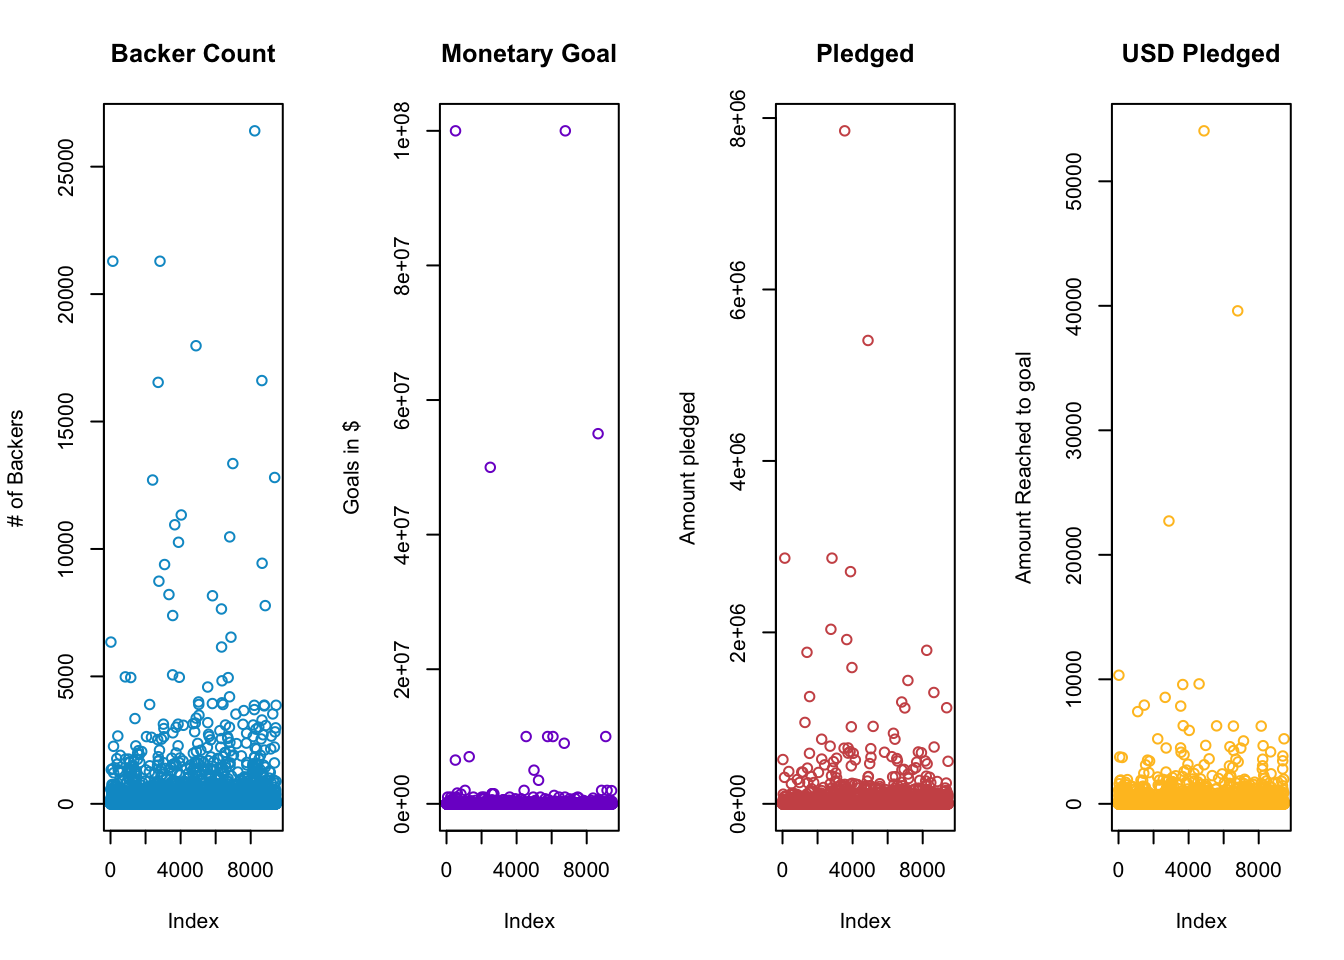
\includegraphics{STAT-382-Final-Project_files/figure-latex/distribution-1.pdf}

\begin{Shaded}
\begin{Highlighting}[]
\KeywordTok{cat}\NormalTok{(}\StringTok{"The quantative variables do not follow any distributions."}\NormalTok{)}
\end{Highlighting}
\end{Shaded}

\begin{verbatim}
## The quantative variables do not follow any distributions.
\end{verbatim}

\hypertarget{e.-show-your-analysis-in-both-tablescharts-and-visually-histograms-qqnorm-plots-boxplots-etc.statistical-modeling}{%
\section{5e. Show your analysis in both tables/charts and visually
(histograms, qqnorm plots, boxplots etc.Statistical
Modeling)}\label{e.-show-your-analysis-in-both-tablescharts-and-visually-histograms-qqnorm-plots-boxplots-etc.statistical-modeling}}

\begin{Shaded}
\begin{Highlighting}[]
\KeywordTok{par}\NormalTok{(}\DataTypeTok{mfrow =} \KeywordTok{c}\NormalTok{(}\DecValTok{3}\NormalTok{,}\DecValTok{3}\NormalTok{)) }\CommentTok{#Creates a 3 x 3 picture of the graphs}

\CommentTok{#Backer Count}
\KeywordTok{hist}\NormalTok{(dataFinal}\OperatorTok{$}\NormalTok{backers_count, }\DataTypeTok{main =} \StringTok{"Backers"}\NormalTok{, }\DataTypeTok{xlab =} \StringTok{"Backer Count"}\NormalTok{)}
\KeywordTok{boxplot}\NormalTok{(dataFinal}\OperatorTok{$}\NormalTok{backers_count)}
\KeywordTok{qqnorm}\NormalTok{(dataFinal}\OperatorTok{$}\NormalTok{backers_count)}
\KeywordTok{qqline}\NormalTok{(dataFinal}\OperatorTok{$}\NormalTok{backers_count)}

\CommentTok{#Goal}
\KeywordTok{hist}\NormalTok{(dataFinal}\OperatorTok{$}\NormalTok{goal, }\DataTypeTok{main =} \StringTok{"Goal"}\NormalTok{)}
\KeywordTok{boxplot}\NormalTok{(dataFinal}\OperatorTok{$}\NormalTok{goal)}
\KeywordTok{qqnorm}\NormalTok{(dataFinal}\OperatorTok{$}\NormalTok{goal)}
\KeywordTok{qqline}\NormalTok{(dataFinal}\OperatorTok{$}\NormalTok{goal)}

\CommentTok{#Pledged}
\KeywordTok{hist}\NormalTok{(dataFinal}\OperatorTok{$}\NormalTok{pledged, }\DataTypeTok{main =} \StringTok{"Pledged"}\NormalTok{)}
\KeywordTok{boxplot}\NormalTok{(dataFinal}\OperatorTok{$}\NormalTok{pledged)}
\KeywordTok{qqnorm}\NormalTok{(dataFinal}\OperatorTok{$}\NormalTok{pledged)}
\KeywordTok{qqline}\NormalTok{(dataFinal}\OperatorTok{$}\NormalTok{pledged)}
\end{Highlighting}
\end{Shaded}

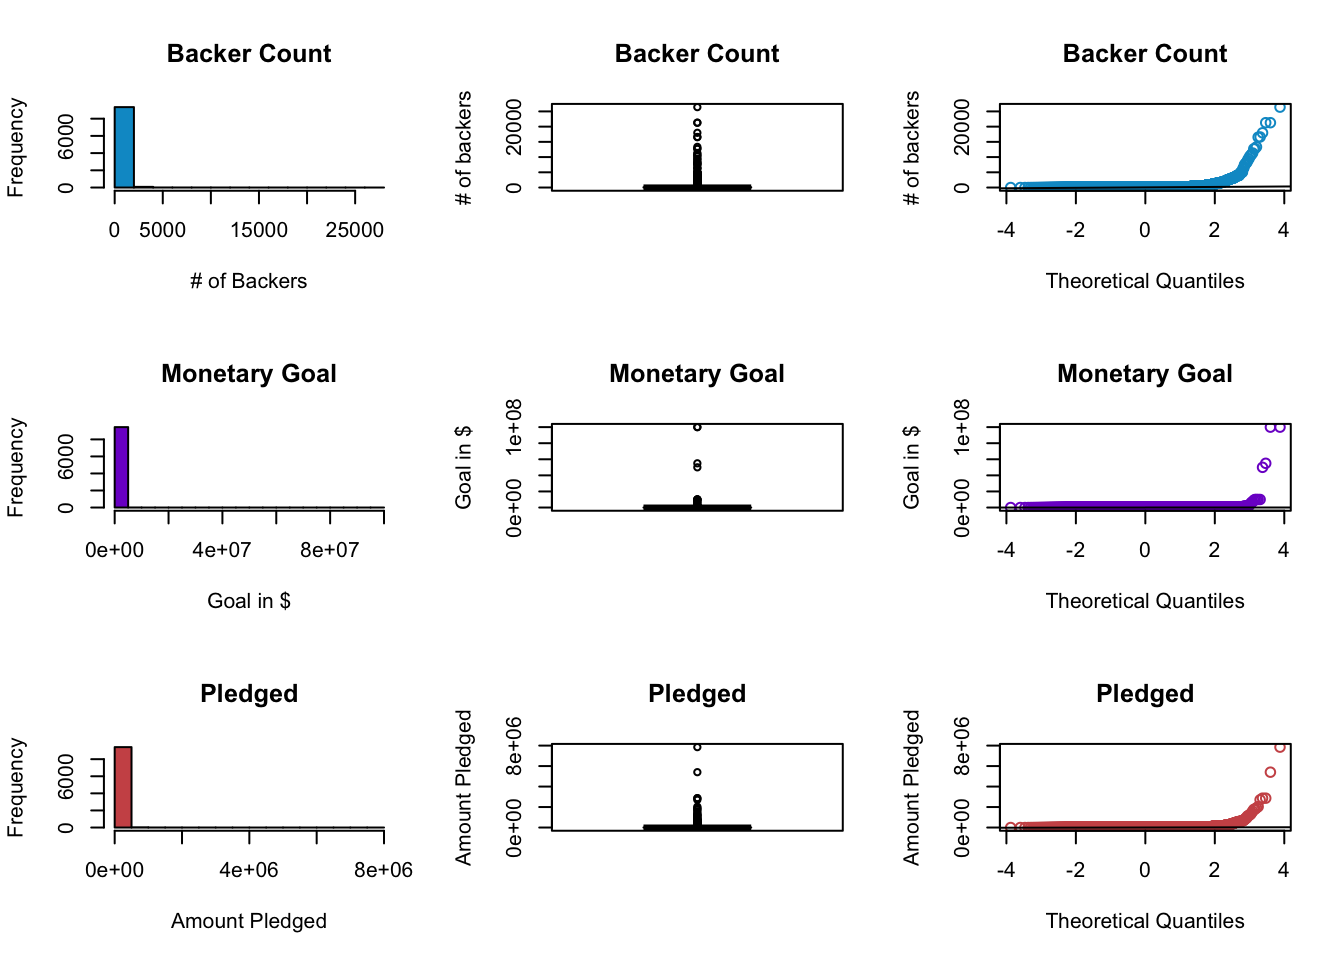
\includegraphics{STAT-382-Final-Project_files/figure-latex/tables/charts and graphs-1.pdf}

\begin{Shaded}
\begin{Highlighting}[]
\KeywordTok{par}\NormalTok{(}\DataTypeTok{mfrow =} \KeywordTok{c}\NormalTok{(}\DecValTok{1}\NormalTok{, }\DecValTok{3}\NormalTok{)) }\CommentTok{#Creates a 2 x 3 picture of the graphs}

\CommentTok{#USD Pledged}
\KeywordTok{hist}\NormalTok{(dataFinal}\OperatorTok{$}\NormalTok{usd_pledged, }\DataTypeTok{main =} \StringTok{"USD Pledged"}\NormalTok{)}
\KeywordTok{boxplot}\NormalTok{(dataFinal}\OperatorTok{$}\NormalTok{usd_pledged)}
\KeywordTok{qqnorm}\NormalTok{(dataFinal}\OperatorTok{$}\NormalTok{usd_pledged)}
\KeywordTok{qqline}\NormalTok{(dataFinal}\OperatorTok{$}\NormalTok{usd_pledged)}
\end{Highlighting}
\end{Shaded}

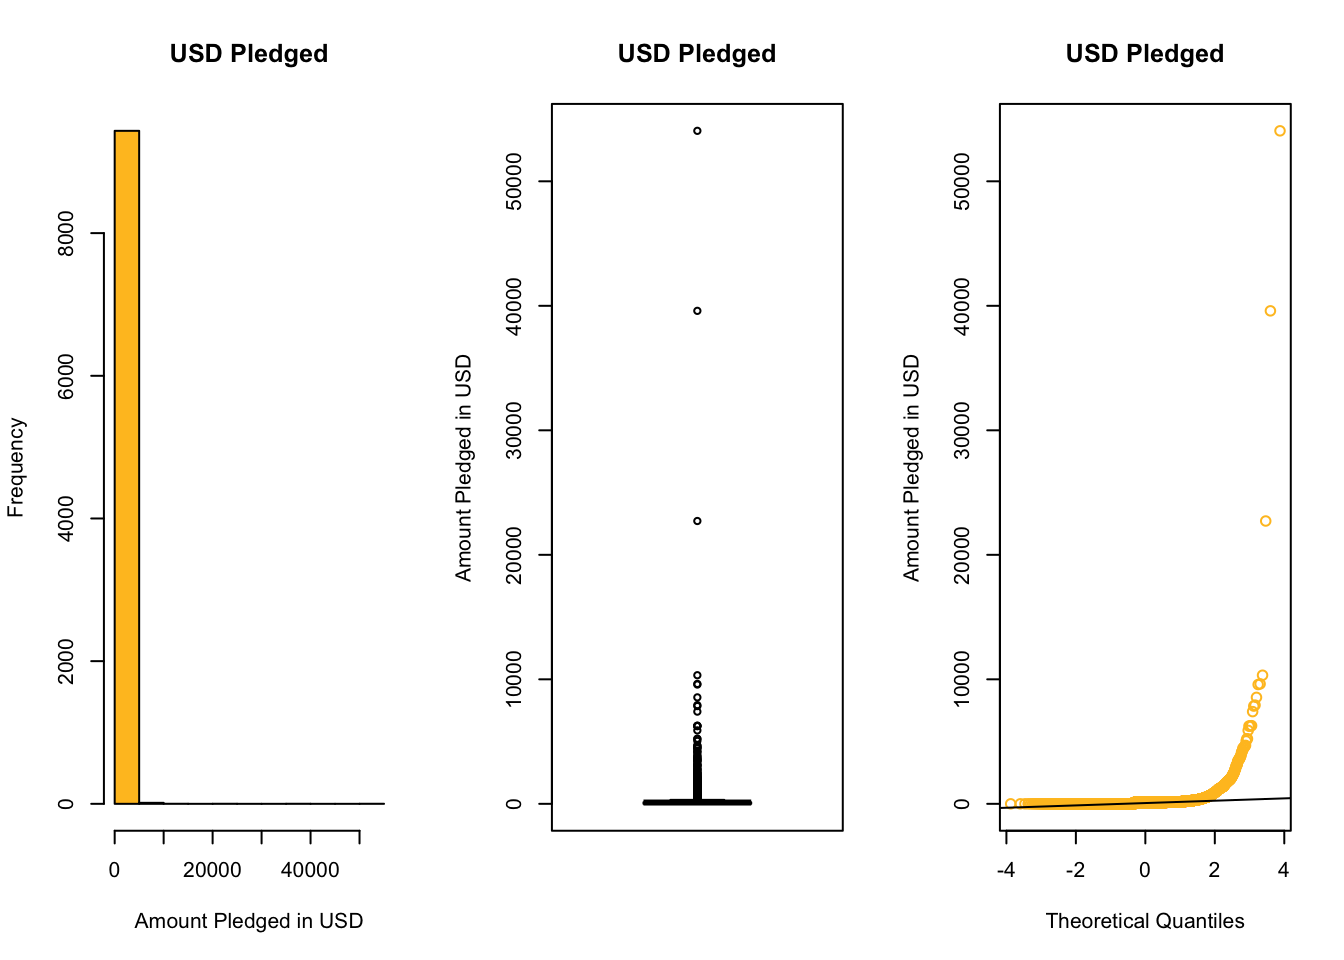
\includegraphics{STAT-382-Final-Project_files/figure-latex/tables/charts and graphs-2.pdf}

\hypertarget{determine-correlations-do-correlation-comparisons-technically-and-visually-use-both-plots-or-pairs-for-your-graphical-representations.-split-your-graphs-in-ways-that-will-help-you-to-conclude-and-infer-based-on-your-model.}{%
\section{6) Determine correlations, do correlation comparisons
(technically and visually ) use both plots or pairs for your graphical
representations. Split your graphs in ways that will help you to
conclude and infer based on your
model.}\label{determine-correlations-do-correlation-comparisons-technically-and-visually-use-both-plots-or-pairs-for-your-graphical-representations.-split-your-graphs-in-ways-that-will-help-you-to-conclude-and-infer-based-on-your-model.}}

The portion above adds a new column labeled ``id''. Every unique item
under category was given a unique id.

\begin{Shaded}
\begin{Highlighting}[]
\KeywordTok{par}\NormalTok{(}\DataTypeTok{mfrow =} \KeywordTok{c}\NormalTok{(}\DecValTok{1}\NormalTok{, }\DecValTok{4}\NormalTok{)) }\CommentTok{#Creates a 1 x 4 picture of the graphs}

\KeywordTok{plot}\NormalTok{(dataFinal}\OperatorTok{$}\NormalTok{id, dataFinal}\OperatorTok{$}\NormalTok{backers_count, }\DataTypeTok{xlab =} \StringTok{"Category"}\NormalTok{, }\DataTypeTok{ylab =} \StringTok{"Backer Count"}\NormalTok{, }\DataTypeTok{main =} \StringTok{"Category vs Backer Count"}\NormalTok{, }\DataTypeTok{col =} \StringTok{"deepskyblue3"}\NormalTok{)}

\KeywordTok{plot}\NormalTok{(dataFinal}\OperatorTok{$}\NormalTok{id, dataFinal}\OperatorTok{$}\NormalTok{goal, }\DataTypeTok{xlab =} \StringTok{"Category"}\NormalTok{, }\DataTypeTok{ylab =} \StringTok{"Goal"}\NormalTok{, }\DataTypeTok{main =} \StringTok{"Category vs Goal"}\NormalTok{, }\DataTypeTok{col =} \StringTok{"deepskyblue3"}\NormalTok{)}

\KeywordTok{plot}\NormalTok{(dataFinal}\OperatorTok{$}\NormalTok{id, dataFinal}\OperatorTok{$}\NormalTok{pledged, }\DataTypeTok{xlab =} \StringTok{"Category"}\NormalTok{, }\DataTypeTok{ylab =} \StringTok{"Pledged"}\NormalTok{, }\DataTypeTok{main =} \StringTok{"Category vs Pledged"}\NormalTok{, }\DataTypeTok{col =} \StringTok{"deepskyblue3"}\NormalTok{)}

\KeywordTok{plot}\NormalTok{(dataFinal}\OperatorTok{$}\NormalTok{id, dataFinal}\OperatorTok{$}\NormalTok{usd_pledged, }\DataTypeTok{xlab =} \StringTok{"Category"}\NormalTok{, }\DataTypeTok{ylab =} \StringTok{"USD Pledged"}\NormalTok{, }\DataTypeTok{main =} \StringTok{"Category vs USD Pledged"}\NormalTok{, }\DataTypeTok{col =} \StringTok{"deepskyblue3"}\NormalTok{)}
\end{Highlighting}
\end{Shaded}

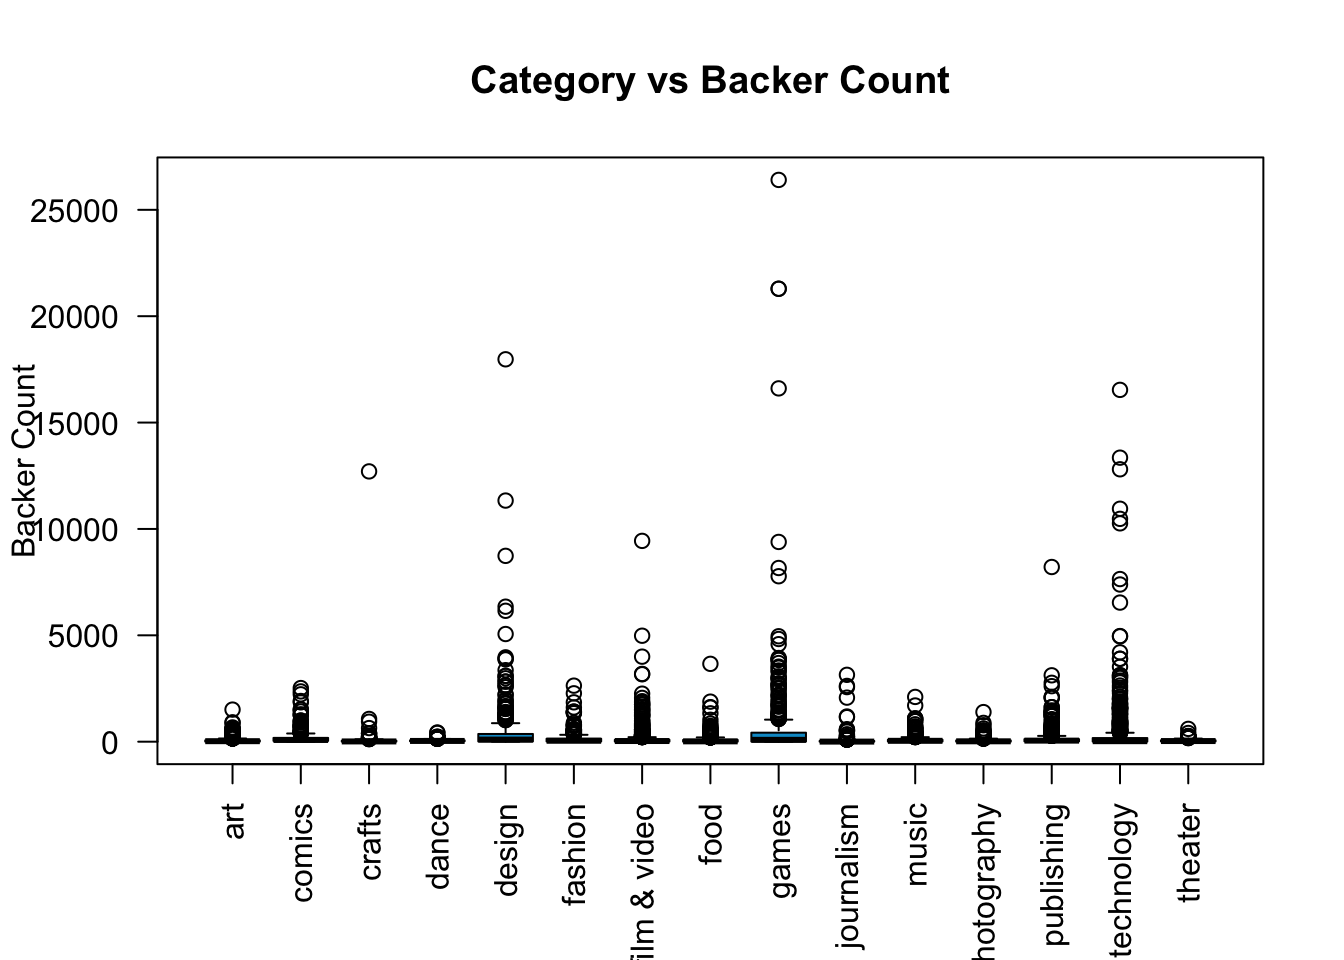
\includegraphics{STAT-382-Final-Project_files/figure-latex/scatter plots-1.pdf}

\begin{Shaded}
\begin{Highlighting}[]
\KeywordTok{pairs}\NormalTok{(}\OperatorTok{~}\NormalTok{dataFinal}\OperatorTok{$}\NormalTok{backers_count }\OperatorTok{+}\StringTok{ }\NormalTok{dataFinal}\OperatorTok{$}\NormalTok{goal }\OperatorTok{+}\StringTok{ }\NormalTok{dataFinal}\OperatorTok{$}\NormalTok{pledged }\OperatorTok{+}\StringTok{ }\NormalTok{dataFinal}\OperatorTok{$}\NormalTok{usd_pledged }\OperatorTok{+}
\StringTok{       }\NormalTok{dataFinal}\OperatorTok{$}\NormalTok{id, }\DataTypeTok{main =} \StringTok{"Backer Count, Goal, Pledged, USD Pledged vs Category"}\NormalTok{)}
\end{Highlighting}
\end{Shaded}

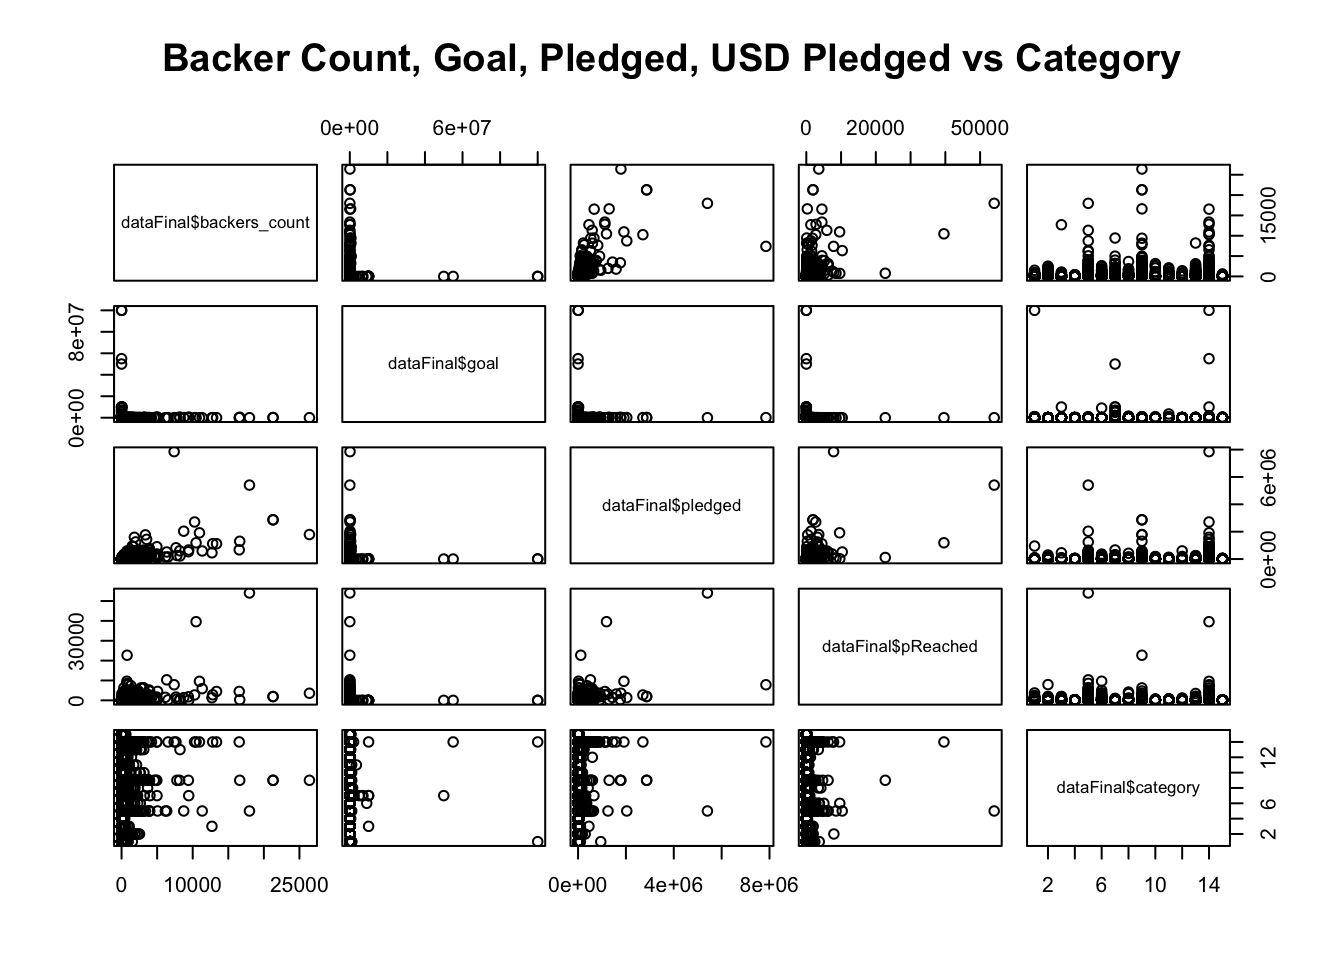
\includegraphics{STAT-382-Final-Project_files/figure-latex/scatter plot matrix-1.pdf}

\begin{Shaded}
\begin{Highlighting}[]
\KeywordTok{cor}\NormalTok{(dataFinal}\OperatorTok{$}\NormalTok{id, dataFinal}\OperatorTok{$}\NormalTok{backers_count)}
\end{Highlighting}
\end{Shaded}

\begin{verbatim}
## [1] -0.05746552
\end{verbatim}

\begin{Shaded}
\begin{Highlighting}[]
\KeywordTok{cor}\NormalTok{(dataFinal}\OperatorTok{$}\NormalTok{id, dataFinal}\OperatorTok{$}\NormalTok{goal)}
\end{Highlighting}
\end{Shaded}

\begin{verbatim}
## [1] -0.002789905
\end{verbatim}

\begin{Shaded}
\begin{Highlighting}[]
\KeywordTok{cor}\NormalTok{(dataFinal}\OperatorTok{$}\NormalTok{id, dataFinal}\OperatorTok{$}\NormalTok{pledged)}
\end{Highlighting}
\end{Shaded}

\begin{verbatim}
## [1] -0.06465228
\end{verbatim}

\begin{Shaded}
\begin{Highlighting}[]
\KeywordTok{cor}\NormalTok{(dataFinal}\OperatorTok{$}\NormalTok{id, dataFinal}\OperatorTok{$}\NormalTok{usd_pledged)}
\end{Highlighting}
\end{Shaded}

\begin{verbatim}
## [1] -0.06465228
\end{verbatim}

\begin{Shaded}
\begin{Highlighting}[]
\KeywordTok{cat}\NormalTok{(}\StringTok{"All of our correlations are negative. This suggests that there is an inverse relationship between category and backer count, goal, pledged, and usd_pledged."}\NormalTok{)}
\end{Highlighting}
\end{Shaded}

\begin{verbatim}
## All of our correlations are negative. This suggests that there is an inverse relationship between category and backer count, goal, pledged, and usd_pledged.
\end{verbatim}

\hypertarget{your-model-and-main-hypothesis-should-be-answered-either-using-anova-or-regression-analysis-or-both.---this-may-mean-depending-on-your-data-that-you-may-need-to-use-a-categorical-variable-to-dissect-your-data-and-that-you-may-need-to-have-data-with-many-more-than-just-2-quantitative-variables.}{%
\section{7) Your model and main hypothesis should be answered either
using ANOVA or Regression Analysis, or both. - This may mean, depending
on your data, that you may need to use a categorical variable to dissect
your data, and that you may need to have data with many more than just 2
quantitative
variables.}\label{your-model-and-main-hypothesis-should-be-answered-either-using-anova-or-regression-analysis-or-both.---this-may-mean-depending-on-your-data-that-you-may-need-to-use-a-categorical-variable-to-dissect-your-data-and-that-you-may-need-to-have-data-with-many-more-than-just-2-quantitative-variables.}}

\#Report The report should be written in R Markdown and then transformed
to HTML. Your report needs to have the following sections:

Introduction - In this section, explain briefly the purpose of your
analysis. Identify your hypothesis, and in a single sentence refer to
the results of your work.

Data - a section describing the data set and how you loaded and
transformed it in R. Include R code blocks within your comments and
explain what the code is doing.

\begin{verbatim}
Analysis - walk through the analysis that you performed. Include R code blocks within your comments and explain what the code is doing.

Issues - Refer to any issues you had with collecting your data, cleaning your data, or implementing your model.

Results - any plots, tables, or other results which gave you the answers to the questions that you were asked. Include R code blocks for any plots and explain what the code is doing.

Discussion - a brief (one or two paragraphs) discussion of the results and how they validate or not your initial claims. 
\end{verbatim}

\begin{Shaded}
\begin{Highlighting}[]
\CommentTok{#Just here to add space}
\end{Highlighting}
\end{Shaded}

\hypertarget{presentation}{%
\section{Presentation}\label{presentation}}

You should prepare a brief (5-8 minutes) presentation on your project

You should create a Powerpoint presentation on your report.

Your Presentation should be narrated, or you should create a recorded
video, presenting the Powerpoint.

\#The presentation should include: Introduction - quick reference to the
problem you are analyzing and your data Hypothesis - main claim or
claims you worked on Methodology - what statistical tools you used to
complete your analysis and why? Issues - any issues you had while you
run your analysis and how did you resolve them Tables, Charts and Graphs
and measures with explanation for your EDA Results of Correlation,
Regression, and ANOVA analysis Conclusions Future questions and further
analysis not addressed in this project References

\end{document}
